% comment out for student version
\ifdefined\Student\relax\else\def\Teacher{}\fi

\documentclass[12pt]{article}

\title{Activity 6: Loops}
\author{Chris Mayfield and Helen Hu}
\date{Spring 2018}

%\ProvidesPackage{cspogil}

% fonts
\usepackage[utf8]{inputenc}
\usepackage[T1]{fontenc}
\usepackage{mathpazo}

% spacing
\usepackage[margin=2cm]{geometry}
\renewcommand{\arraystretch}{1.4}
\setlength{\parindent}{0pt}

% orphans and widows
\clubpenalty=10000
\widowpenalty=10000
\pagestyle{empty}

% figures and tables
\usepackage{graphicx}
\usepackage{multicol}
\usepackage{tabularx}
\usepackage{wrapfig}

% fixed-width columns
\usepackage{array}
\newcolumntype{L}[1]{>{\raggedright\let\newline\\\arraybackslash\hspace{0pt}}m{#1}}
\newcolumntype{C}[1]{>{\centering\let\newline\\\arraybackslash\hspace{0pt}}m{#1}}
\newcolumntype{R}[1]{>{\raggedleft\let\newline\\\arraybackslash\hspace{0pt}}m{#1}}

% include paths
\makeatletter
\def\input@path{{Models/}{../../Models/}}
\graphicspath{{Models/}{../../Models/}}
\makeatother

% colors
\usepackage[svgnames,table]{xcolor}
\definecolor{bgcolor}{HTML}{FAFAFA}
\definecolor{comment}{HTML}{007C00}
\definecolor{keyword}{HTML}{0000FF}
\definecolor{strings}{HTML}{B20000}

% table headers
\newcommand{\tr}{\bf\cellcolor{Yellow!10}}

% syntax highlighting
\usepackage{textcomp}
\usepackage{listings}
\lstset{
    basicstyle=\ttfamily\color{black},
    backgroundcolor=\color{bgcolor},
    numberstyle=\scriptsize\color{comment},
    commentstyle=\color{comment},
    keywordstyle=\color{keyword},
    stringstyle=\color{strings},
    columns=fullflexible,
    keepspaces=true,
    showlines=true,
    showstringspaces=false,
    upquote=true
}

% code environments
\newcommand{\java}[1]{\lstinline[language=java]{#1}}%[
\lstnewenvironment{javalst}{\lstset{language=java,backgroundcolor=}}{}
\lstnewenvironment{javabox}{\lstset{language=java,frame=single,numbers=left}\quote}{\endquote}

% PDF properties
\usepackage[pdftex]{hyperref}
\urlstyle{same}
\makeatletter
\hypersetup{
  pdftitle={\@title},
  pdfauthor={\@author},
  pdfsubject={\@date},
  pdfkeywords={},
  bookmarksopen=false,
  colorlinks=true,
  citecolor=black,
  filecolor=black,
  linkcolor=black,
  urlcolor=blue
}
\makeatother

% titles
\makeatletter
\renewcommand{\maketitle}{\begin{center}\LARGE\@title\end{center}}
\makeatother

% boxes [optional height]
\newcommand{\emptybox}[1][10em]{
\vspace{1em}
\begin{tabularx}{\linewidth}{|X|}
\hline\\[#1]\hline
\end{tabularx}}

% models
\newcommand{\model}[1]{\section{#1}\nopagebreak}
\renewcommand{\thesection}{Model~\arabic{section}}

% questions
\newcommand{\quest}[1]{\subsection*{Questions~ (#1)}}
\newcounter{question}
\newcommand{\Q}{\vspace{1em}\refstepcounter{question}\arabic{question}.~ }
\renewcommand{\thequestion}{\#\arabic{question}}

% sub-question lists
\usepackage{enumitem}
\setenumerate[1]{label=\alph*)}
\setlist{itemsep=1em,after=\vspace{1ex}}

% inline answers
\definecolor{answers}{HTML}{C0C0C0}
\newcommand{\ans}[1]{%
\ifdefined\Student
    \leavevmode\phantom{~~\textcolor{answers}{#1}}
\else
    ~~\textcolor{answers}{#1}
\fi}

% longer answers [optional height]
\newsavebox{\ansbox}
\newenvironment{answer}[1][4em]{
\nopagebreak
\begin{lrbox}{\ansbox}
\begin{minipage}[t][#1]{\linewidth}
\color{answers}
}{
\end{minipage}
\end{lrbox}
\ifdefined\Student
    \phantom{\usebox{\ansbox}}%
\else
    \usebox{\ansbox}%
\fi}


\begin{document}

\maketitle

Computers are often used to perform repetitive tasks.
Running the same statements over and over again, without making any mistakes, is something that computers do very well.

\guide{
  \item Explain what happens when re-assigning a variable.
  \item Identify the three main components of a while loop.
  \item Implement the factorial function using a for loop.
}{
  \item Tracing the execution of while/for loops and predict their final output. (Critical Thinking)
}{
\ref{assignment.tex} addresses two misconceptions about assignment: what happens when you reassign a variable, and how do you swap two variables. This understanding is essential for loop updates.

Consider bringing a pair of note cards labeled with a large 1 on the first and a large 2 on the second card.
Have all team members put one hand behind their back, and then hand the cards to two students (student $X$ gets the 1 and student $Y$ gets the 2).
Ask them to exchange cards, and if they struggle, say ``What if you had a student $Z$ who could help?''
(Credit: Debra Duke)

When reporting out \ref{while-loops.tex}, have teams predict the answers to \ref{output}, \ref{value}, and \ref{do99}.
Then execute the code and have them discuss their results, if incorrect.
Consider stepping through the code with a debugger (on the projector) during report-out.

Be sure to make connections between the flow charts in \ref{while-loops.tex} and \ref{for-loops.tex}.
You may need to guide students on \ref{forchar} applying string methods in the context of a loop.
On \ref{nested}, students might not think to use a {\tt long} variable to store the factorial.
If time permits, show the output of the solution with {\tt fact} declared as an {\tt int}, and ask them to fix the code.
}

\model{Assignment}
% based on Model 2 of Activity 08 - Introduction to Loops by Helen Hu

Consider the following Java statements. What is the resulting value of each variable?

\begin{center}
\vspace{-6pt}
\begin{tabular}{cp{120pt}cp{120pt}cp{120pt}}

\textsf{A:}
&
\vspace{-1em}
\begin{javalst}
int x, y;
x = 1;
y = 2;
y = x;
x = y;

\end{javalst}

&
\textsf{B:}
&
\vspace{-1em}
\begin{javalst}
int x, y, z;
x = 1;
y = 2;
z = y;
y = x;
x = z;
\end{javalst}

&
\textsf{C:}
&
\vspace{-1em}
\begin{javalst}
int z, y;
z = 2;
z = z + 1;
z = z + 1;
y = y + 1;

\end{javalst}

\\[-1em]
&
Value of x: \ans[3em]{1}

\vspace{1em}
Value of y: \ans[3em]{1}

&
&
Value of x: \ans[3em]{2}

\vspace{1em}
Value of y: \ans[3em]{1}

\vspace{1em}
Value of z: \ans[3em]{2}

&
&
Value of z: \ans[3em]{4}

\vspace{1em}
Value of y: \ans[3em]{?}

\end{tabular}
\vspace{-14pt}
\end{center}


\quest{10 min}


\Q In program~\textsf{A}, why is the value of \java{x} not 2?

\begin{answer}[3em]
Each statement is executed one after the other, so the third assignment changes the value of \java{y} to 1.
The last assignment then assigns 1 to the value \java{x}.
\end{answer}


\Q In program~\textsf{B}, what happens to the values of \java{x} and \java{y}?

\begin{answer}[3em]
They get swapped; \java{x} was 1 and \java{y} was 2, but in the end \java{x} was 2 and \java{y} was 1.
\end{answer}


\Q In program~\textsf{B}, what is the purpose of the variable \java{z}?

\begin{answer}[3em]
It is a temporary variable that makes it possible to swap the values of \java{x} and \java{y}.
\end{answer}


\Q If program~\textsf{C} runs, what happens to the value of \java{z}?

\begin{answer}[3em]
It gets incremented twice; the value starts at 2, then it becomes 3, and then it becomes 4.
\end{answer}


\Q In program~\textsf{C}, why is it possible to increment \java{z} but not \java{y}?

\begin{answer}[3em]
The variable \java{z} was initialized, but \java{y} was not.
Java doesn't know what value to increment.
\end{answer}


\Q Because \emph{increment} and \emph{decrement} are so common in algorithms, Java provides the operators \java{++} and \java{--}.
For example, ~\java{x++} is the same as ~\java{x = x + 1}, and \java{y--} is the same as ~\java{y = y - 1}.
Write the value of \java{x} and \java{y} next to each statement below.

\vspace{-1ex}
\begin{center}
\begin{minipage}{90pt}
\begin{javalst}
int x = 5;
x--;
x--;
\end{javalst}
\end{minipage}
\begin{minipage}{100pt}
\begin{answer}[3.5em]
\begin{javaans}
x is 5
x is 4
x is 3
\end{javaans}
\end{answer}
\end{minipage}
\hspace{3em}
\begin{minipage}{90pt}
\begin{javalst}
int y = -10;
y++;
y++;
\end{javalst}
\end{minipage}
\begin{minipage}{100pt}
\begin{answer}[3.5em]
\begin{javaans}
y is -10
y is -9
y is -8
\end{javaans}
\end{answer}
\end{minipage}
\end{center}
\vspace{-1em}


\Q \label{compound}
Like the assignment operator, the \java{++} and \java{--} operators replace the value of a variable.
Java also has \emph{compound assignment} operators for convenience.
For example, the statement ~\java{x = x + 2} can be rewritten as ~\java{x += 2}.
Simplify the following assignment statements.

\vspace{-1ex}
\begin{center}
\begin{minipage}{150pt}
\begin{javalst}
step = step + 5;
size = size - 3;
total = total * 2;
change = change / 10;
hours = hours % 24;
\end{javalst}
\end{minipage}
\begin{minipage}{150pt}
\begin{answer}[6em]
\begin{javaans}
step += 5;
size -= 3;
total *= 2;
change /= 10;
hours %= 24;
\end{javaans}
\end{answer}
\end{minipage}
\end{center}
\vspace{-1em}


\Q Which of the following assignment statements can also be rewritten like the ones in \ref{compound}?

\vspace{-1ex}
\begin{center}
\begin{minipage}{150pt}
\begin{javalst}
step = 5 + step;
size = 3 - size;
total = 2 * total;
change = 10 / change;
hours = 24 % hours;
\end{javalst}
\end{minipage}
\begin{minipage}{150pt}
\begin{answer}[6em]
\begin{javaans}
step += 5;
NO
total *= 2;
NO
NO
\end{javaans}
\end{answer}
\end{minipage}
\end{center}
\vspace{-1em}

\vfill
\model{While Loops}

A loop is a set of instructions that are to be repeated.
All loops have three main components: \emph{initialize}, \emph{test}, and \emph{update}.
Label each of these components in the two example loops below.

\vspace{1ex}
\begin{javalst}
    // pre-test loop                         // post-test loop
    number = 1;                              number = 1;
    while (number <= 10) {                   do {
        System.out.println(number);              System.out.println(number);
        number++;                                number++;
    }                                        } while (number <= 10);
\end{javalst}

\vspace{2pt}
\hspace{3em}
\raisebox{0.5em}{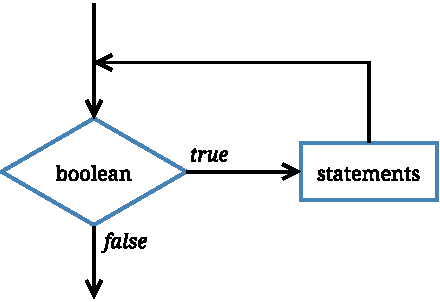
\includegraphics[height=9em]{while.pdf}}
\hspace{9em}
\raisebox{0em}{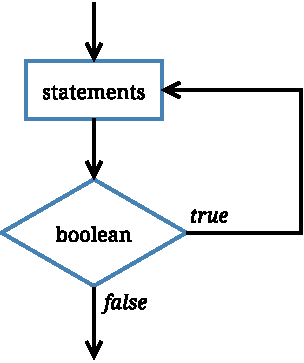
\includegraphics[height=10em]{dowhile.pdf}}


\quest{15 min}


\Q Which loop component always happens first? Why?

\begin{answer}
The initialize step; you need to tell the loop where to begin.
And variables cannot be updated until they have an initial value.
\end{answer}


\Q Explain why the \java{while} loop is called a \emph{pre-test} and the \java{do while} loop is called a \emph{post-test}.

\begin{answer}
The \texttt{while} tests its condition before the loop body, whereas the \texttt{do while} tests its condition after the loop body.
\end{answer}


\Q \label{output}
What is output (to the screen) by each loop?

\begin{answer}
They both print the numbers 1 through 10, with each number on its own line.
\end{answer}


\Q \label{value}
What is the final value of \java{number} at the end of each loop?

\begin{answer}
At the end of each loop, the value of \java{number} is 11.
\end{answer}


\Q What is output if you swap the \java{println} and \java{number++} statements?

\begin{answer}
Both loops print the values 2 through 11 instead.
\end{answer}


\Q What is the output if you remove the \java{number++} statement?

\begin{answer}
Both loops will print the value 1 forever, since \java{number} never reaches the stopping condition.
\end{answer}


\Q \label{do99}
What is output by the loop below?

\begin{minipage}{0.49\textwidth}
\begin{javalst}
    number = 99;
    do {
        System.out.println(number);
        number++;
    } while (number <= 10);
    System.out.println(number);
\end{javalst}
\end{minipage}
\hfill
\begin{minipage}{0.49\textwidth}
\begin{answer}
It will print the numbers 99 and 100; the \texttt{do while} loop does not repeat since 99 is greather than 10.
\end{answer}
\end{minipage}
\vspace{1ex}


\Q What is the output of the following loop? (And what mistake was made?)

\begin{minipage}{0.49\textwidth}
\begin{javalst}
    i = 0;
    while (i < 3) 
        System.out.println("n = " + i);
        i = i + 1;
\end{javalst}
\end{minipage}
\hfill
\begin{minipage}{0.49\textwidth}
\begin{answer}
It will print \texttt{"n = 3"} forever. Without braces, the loop only executes the first statement, and ~\java{i = i + 1;} is never reached.
\end{answer}
\end{minipage}
\vspace{1ex}


\Q What is the difference between a \java{while} statement and an \java{if} statement?

\begin{answer}
They identical syntax and a similar meaning; the only difference is a \texttt{while} statement repeats the code between its braces as long as the condition is \texttt{true}.
\end{answer}

\model{For Loops}

The for loop combines \emph{initialize}, \emph{test}, and \emph{update} into one line of code.
Label each of these components in the two example loops below.
(Assume that the variable \java{number} has already been declared.)

\vspace{1ex}
\begin{minipage}{0.6\linewidth}
\begin{javalst}
    // count forwards
    for (number = 1; number <= 10; number++) {
        System.out.println(number);
    }

    // count backwards
    for (number = 10; number >= 1; number--) {
        System.out.println(number);
    }
\end{javalst}
\end{minipage}
\hfill
\begin{minipage}{0.38\linewidth}
\centering
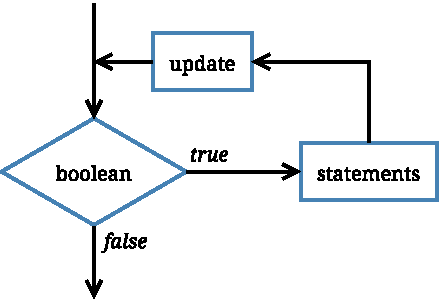
\includegraphics[height=10em]{for.pdf}
\end{minipage}

\quest{20 min}


\Q What do each of the \java{for} loops output to the screen? Be specific.

\begin{answer}
The first loop prints the numbers 1 to 10, and the second loop prints the numbers 10 to 1.
Each number is on its own line.
\end{answer}


\Q Describe how to make these loops display even numbers only (2 4 6 8 10 and 10 8 6 4 2).

\begin{answer}
Change the first loop: ~\texttt{for (number = 2; number <= 10; number += 2)}.

Change the second loop: ~\texttt{for (number = 10; number >= 2; number -= 2)}.
\end{answer}


\Q \label{forchar}
Write a \java{for} loop that prints each character of a string on a separate line.
You will need to invoke the \java{length()} and \java{charAt()} methods.
Assume the string variable is named \java{word}.

\begin{answer}
\vspace{-1ex}
\begin{javaans}
    for (int i = 0; i < word.length(); i++) {
        System.out.println(word.charAt(i));
    }
\end{javaans}
\end{answer}


\Q Rewrite your \java{for} loop in \ref{forchar} as a \java{while} loop.

\begin{answer}[6em]
\vspace{-1ex}
\begin{javaans}
    int i = 0;
    while (i < word.length()) {
        System.out.println(word.charAt(i));
        i++;
    }
\end{javaans}
\end{answer}


\Q Write a loop that computes the factorial of a given integer \java{n}.
Recall that $n! = n * (n-1) * (n-2) * \ldots * 1$.
Store your result in a variable named \java{fact}.

\begin{answer}[6em]
\vspace{-1ex}
\begin{javaans}
    long fact = 1;  // not int
    for (int i = n; i > 1; i--) {
        fact *= i;
    }
\end{javaans}
\end{answer}


\Q \label{nested}
A \emph{nested loop} is one that exists within the scope of another loop.
This construct is often used when there are two variables for which all combinations must be examined.

\begin{javalst}
    for (int i = 0; i < 10; i++) {
        for (int j = 0; j < 10; j++) {
            System.out.printf("The product of %d and %d is %d\n", i, j, i * j);
        }
        System.out.println();
    }
\end{javalst}

Write nested loops that compute and display the factorial of each integer from 1 to 20.
(Reuse your code from the previous question.)
Your output should be in this format:

\vspace{-1ex}
\begin{verbatim}
    The factorial of 1 is 1
    The factorial of 2 is 2
    The factorial of 3 is 6
    The factorial of 4 is 24
\end{verbatim}
\vspace{-3ex}

\begin{answer}[10em]
\begin{javaans}
    for (int n = 1; n <= 20; n++) {
        long fact = 1;  // not int
        for (int i = n; i > 1; i--) {
            fact *= i;
        }
        System.out.printf("The factorial of %d is %d\n", n, fact);
    }
\end{javaans}
\end{answer}


\end{document}
